\begin{activity}{Thermal Diffusivity, Thermal Length, and Timescales}

\section*{Purpose}
To understand transient heat flow in terms of:
\begin{itemize}
  \item how far thermal signals propagate in a given time,
  \item how long it takes thermal changes to affect a given depth,
  \item and how the \emph{thermal length scale} controls signal shape and timing.
\end{itemize}

{\color{red}
\section*{Learning Outcomes}

By the end of this activity, you should be able to:
\begin{itemize}
  \item Define thermal diffusivity and explain which material properties control it.
  \item Use the thermal length scale $\ell_T = 2\sqrt{\kappa t}$ to estimate how far a thermal signal has propagated or how long it takes to reach a given depth.
  \item Interpret the error function solution qualitatively and identify where temperature changes are largest.
  \item Compare thermal diffusion timescales for different materials (ice, sediment, granite, mantle) and connect these to geological processes.
\end{itemize}
}

\section*{Background}
Thermal diffusivity is defined as
\[
\kappa = \frac{k}{\rho c_p},
\]
where $k$ is thermal conductivity, $\rho$ is density, and $c_p$ is specific heat.

\begin{table}
    \centering
    \begin{tabular}{lccc}
        \toprule
        \textbf{Material} &
        \textbf{Thermal Conductivity $k$} &
        \textbf{Thermal Diffusivity $\kappa$} &
        \textbf{Thermal Diffusivity $\kappa$} \\
        &
        \textbf{(W m$^{-1}$ K$^{-1}$)} &
        \textbf{(m$^2$ s$^{-1}$)} &
        \textbf{(km$^2$ My$^{-1}$)} \\
        \midrule
        Ice (glacial / ice sheet average) &
        1.6--2.0 &
        $(0.7$--$0.9)\times10^{-6}$ &
        22--28 \\

        Clay-rich sediments &
        0.6--1.5 &
        $(0.2$--$0.5)\times10^{-6}$ &
        6--16 \\

        Granite &
        2.5--3.5 &
        $(0.8$--$1.2)\times10^{-6}$ &
        25--38 \\

        Basalt / Gabbro &
        1.7--2.2 &
        $(0.6$--$1.0)\times10^{-6}$ &
        19--32 \\

        Peridotite (upper mantle) &
        3.3--4.5 &
        $(1.0$--$1.5)\times10^{-6}$ &
        32--47 \\
        \bottomrule
    \end{tabular}
\end{table}

\smallskip
\noindent
\textit{Values are representative ranges. Thermal conductivity and diffusivity
vary with temperature, porosity, mineralogy, fluid content, and fabric.
Diffusivities are calculated using $\kappa = k/(\rho c_p)$ and rounded for
scaling arguments rather than precise modeling.}

For diffusion-dominated heat transfer, the characteristic depth over which temperature changes propagate scales as
\[
z \sim 2 \sqrt{\kappa t}.
\]

This thermal length sets both:
\begin{itemize}
  \item the depth to which temperature changes have propagated after time $t$,
  \item the timescale required for a thermal perturbation at depth to influence
  shallower levels.
\end{itemize}

\section*{Error Function Solution}

For instantaneous heating or cooling at a boundary, the temperature evolution is given by the error function solution:
\[
T(z,t) = T_s + (T_b - T_s)\,
\erf \left(\frac{z}{2\sqrt{\kappa t}}\right).
\]

\textbf{Important:}  
The argument of the error function,
\[
\eta = \frac{z}{2\sqrt{\kappa t}},
\]
controls the \emph{shape and timing} of the thermal signal.



\section*{Tasks}
\begin{enumerate}
  \item For timescales of $10^3$, $10^5$, and $10^7$ years, describe how the depth of thermal influence would differ between rock and ice.
  \answerbox[3cm]

  \item Explain why borehole paleothermometry in rock requires much greater depths to recover long-term climate signals than ice-core records.
  \answerbox[3cm]
\end{enumerate}

\section*{Tasks}

\subsection*{A. Distance Given Time}
\begin{enumerate}
  \item For a fixed time $t$, describe how temperature varies with depth $z$ as
  the value of $\eta$ increases.
  \answerbox[2cm]

  \item Explain why temperature changes are largest for $\eta \ll 1$ and become
  negligible for $\eta \gg 1$.
  \answerbox[2cm]

  \item Using the thermal length $\ell_T$, estimate the depth to which a surface
  temperature change has propagated after a given time.
  \answerbox[2cm]
\end{enumerate}

\subsection*{B. Time Given Distance}
\begin{enumerate}
  \item Rearranging the thermal length relation,
  \[
  t \sim \frac{z^2}{\kappa},
  \]
  explain what sets the timescale for heat to travel a distance $z$.
  \answerbox[2cm]

  \item Consider a plume impinging on the base of the lithosphere.
  If the lithosphere is $x$ km thick, what controls how long it takes for this
  thermal perturbation to influence surface temperatures?
  \answerbox[2cm]

  \item Following delamination of a dense crustal root, heat is supplied from
  below. Explain why crustal heating is delayed rather than instantaneous.
  \answerbox[2cm]
\end{enumerate}

\subsection*{C. Interpreting ``Arrival'' of Heat}
\begin{enumerate}
  \item Does heat arrive at a specific time, or does it diffuse gradually?
  Use the error function shape to justify your answer.
  \answerbox[2cm]

  \item For $\eta \approx 1$, what fraction of the total temperature change has
  occurred? What does this imply about defining a thermal response time?
  \answerbox[2cm]

  \item Discuss why the concept of a sharp thermal front is inappropriate for
  diffusion-dominated heat transport.
  \answerbox[2cm]
\end{enumerate}

\section*{Geological Interpretation}

\begin{itemize}
  \item Thick lithosphere acts as a strong thermal filter, delaying surface
  response to basal heating.
  \item Thermal signals generated at depth are attenuated and spread in time as
  they propagate upward.
  \item The thermal length scale controls which geological processes can be
  observed at the surface and on what timescales.
\end{itemize}

\section*{Key Idea}

\vspace{0.5em}

\noindent
\fbox{
\parbox{0.93\textwidth}{
In diffusion problems, time and distance are interchangeable through the
thermal length $\ell_T = 2\sqrt{\kappa t}$.
Heat does not ``arrive'' at a depth at a single moment; instead, the error function
describes a gradual, scale-dependent thermal response controlled by diffusivity,
distance, and boundary conditions.
}
}

{\color{blue}
\begin{figure}[h]
\centering
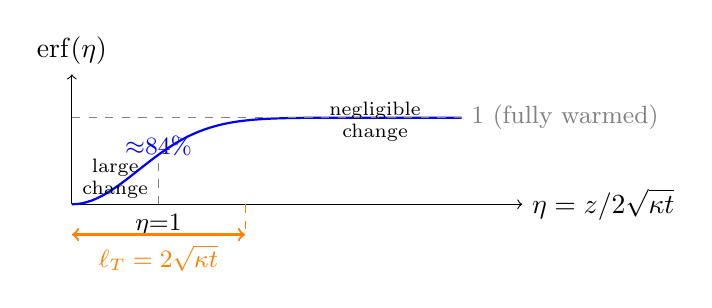
\begin{tikzpicture}[scale=1.1]
  % axes
  \draw[->] (0,0) -- (5.2,0) node[right] {$\eta = z/2\sqrt{\kappa t}$};
  \draw[->] (0,0) -- (0,1.5) node[above] {$\mathrm{erf}(\eta)$};

  % erf curve (approximate via tanh-like shape)
  \draw[thick, blue, domain=0:4.5, samples=80]
    plot (\x, {1.0 - exp(-\x*\x*0.85)});

  % Annotations
  \draw[dashed, gray] (0, 1.0) -- (4.5, 1.0) node[right, font=\small] {1 (fully warmed)};
  \draw[dashed, gray] (1.0, 0) -- (1.0, {1.0 - exp(-0.85)});
  \node[font=\small, below] at (1.0, 0) {$\eta{=}1$};
  \node[font=\small, blue] at (1.0, {1.0 - exp(-0.85)+0.1}) {${\approx}84\%$};

  % Thermal length marker
  \draw[<->, thick, orange] (0, -0.35) -- (2.0, -0.35)
    node[midway, below, font=\small] {$\ell_T = 2\sqrt{\kappa t}$};
  \draw[dashed, orange] (2.0, 0) -- (2.0, -0.35);

  % Region labels
  \node[font=\scriptsize, align=center] at (0.5, 0.3) {large \\ change};
  \node[font=\scriptsize, align=center] at (3.5, 0.95) {negligible \\ change};
\end{tikzpicture}
\caption{The error function $\mathrm{erf}(\eta)$ describes the gradual thermal response to a surface temperature change. The thermal length $\ell_T = 2\sqrt{\kappa t}$ marks the depth of significant influence ($\eta = 1$, approximately 84\% of the total change).}
\end{figure}
}

\end{activity}